\documentclass[norsk]{article}
\usepackage[utf8]{inputenc}
\usepackage{graphicx}
\usepackage{enumitem}

%Sets the languages
\usepackage[norsk, english]{babel}

%Configuration of numbered list
\newlist{legal}{enumerate}{10}
\setlist[legal]{label*=\arabic*.}


\title{Kravspesifikasjon}
\author{}
\date{Oktober 2019}

\begin{document}

\maketitle

\section{Introduksjon}

\section{Krav}
\subsection{Funksjonelle krav}
\begin{legal}
    \item Webside
    \begin{legal}
        \item Alle skal kunne se kalender for inneværende måned med arrangementer og trykke seg tilbake til forrige måned eller frem til neste måned.
        \item Alle skal kunne laste ned kalenderdata. 
        \item Alle skal kunne se kalenderdata på websiden.
        \item Alle skal kunne spesifisere ønsket sport som vises i kalender.
        \item Alle skal kunne søker etter arrangementer
        \item Alle skal kunne søke etter terminlister.
        \item Alle skal kunne søke i terminlister.
        \item Alle skal kunne søke etter klubber.
        \item Alle skal kunne søke etter utøveres profil. 
        \item En klubb skal kunne vise utøverdata.
        \begin{legal}
            \item Utøverdata skal bestå av navn og bilde.
        \end {legal}
        \item Alle skal kunne se detaljer om arrangementer.
        \item Ingen brukere skal kunne logge seg inn 
        i webgrensesnittet.
    \end{legal}
    \item Applikasjon
    \begin{legal}
        \item Klubb og administrator skal kunne logge inn på  applikasjonen ved hjelp av å trykke på en knapp.
        \item Etter innlogging skal en meny med knapper vises for klubb og admin
        \begin{legal}
            \item Menyens innhold avhenger av brukerstatus.
        \end{legal}
        \item Klubb skal kunne legge til kommende arrangementer.
        \item En klubb skal kunne legge inn utøverdata.
        \item Klubb skal ikke kunne slette overståtte arrangementer.
        \item Applikasjonen skal kunne skalere etter brukeren sin enhetsstørrelse.
        \item Bruker skal kunne laste ned kalender data.
        \item Klubb skal kunne registrere utøvers resultater
        \item En klubb skal kunne registrere medlemmer
        \begin{legal}
            \item En klubb skal kunne dele inn medlemmer i lag/aldersgrupper
            \item En klubb skal kunne redigere medlemmer
        \end{legal}
        \item I registrering av medlemmer til et arrangement skal medlemmer velges via en dropdown-meny
    \end{legal}
    \item API
    \begin{legal}
        \item Systemet skal kunne ta i mot tabeller med data og importere det til database (på hvilket format?)
        \item Systemet skal bare gi lese rettigheter til webside.
    \end{legal}
    
    \subsection{Ikke-funksjonelle krav}
    \item Applikasjon
    \begin{legal}
        \item Kalenderdata skal kunne bli synkronisert med Google Calendar-API
        \item GUI skal være enkelt å bruke
    \end{legal}
    \item Database
    \begin{legal}
        \item Databasen skal kjøre MySQL
        \item Passord lagres hashet og saltet (og pepret)
        \item Databasen skal leve i en skytjeneste
        \item Databasen skal være rask
        
    \end{legal}
    \item Brukere
    \begin{legal}
        \item Sluttbruker (hvem er sluttbruker?)
        \item Klubb
        \item Admin
    \end{legal}
    
    \item Administrator
\end{legal}

\section{Prosjektets tidsestimater}
Prosjektets krav er blitt estimert for å bedre kunne prioritere og delegere arbeidsoppgaver. Nedenfor finner du tabeller sortert etter krav, med tilhørende tidsestimat og prioritet.\newline
Tidsestimat og prioritet er gitt ved t-skjorte størrelser. Dette gjør det lettere for teamet å kunne sortere arbeidsoppgaver etter omfang uten at man føler seg bundet av at en oppgave skal ta et spesifikt anatall timer eller dager. Estimering av antall timer er umulig og det blir derfor nyttigere å gi arbeidsoppgaver en tidsfrist i stedet.
\subsection{Nettsted}
\begin{table}[h]
\begin{tabular}{|l|l|l|}
\hline
Krav              & Tidsestimat & Prioritet \\ \hline
1.1-1.4 & M           & L         \\ \hline
1.1-1.9     & S           & S         \\ \hline
1.10              & S           & S         \\ \hline
1.11              & M           & M         \\ \hline
\end{tabular}
\end{table}
\subsection{Java-applikasjon}
\begin{table}[h]
\begin{tabular}{|l|l|l|}
\hline
Krav & Tidsestimat & Forretningsnytte \\ \hline
2.1  & S           & L               \\ \hline
2.2  & S           & S               \\ \hline
2.3  & L           & L               \\ \hline
2.4  & M           & S               \\ \hline
2.6  & S           & M               \\ \hline
2.7  & S           & M               \\ \hline
2.8  & S           & L               \\ \hline
2.9  & S           & M               \\ \hline
2.10 & S           & L               \\ \hline
\end{tabular}
\end{table}

\section{Sekvensdiagram}
\subsection{Registrere utøvers resultater}

\begin{figure}[ht]
\centering 
    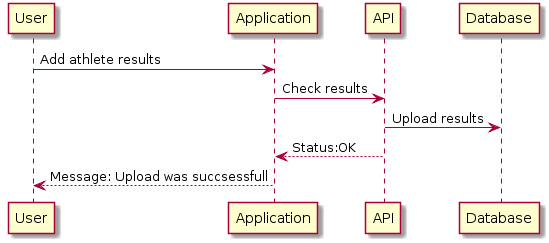
\includegraphics[scale=0.6]{images/add-athlete-results}
    \caption{Sekvensdiagram for å registrere utøvers resultater}\label{fig:add-at-res}
\end{figure}
\subsection{Populere resultater fra arrangement på nettsted}
\begin{figure}[ht]
\centering 
    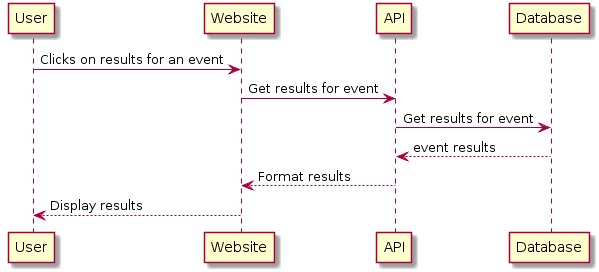
\includegraphics[scale=0.5]{images/get-athletes}
    \caption{Sekvensdiagram for henting av resultater fra arrangement}\label{fig:get-at-res}
\end{figure}

\subsection{API kall}
\begin{figure}[ht]
\centering 
    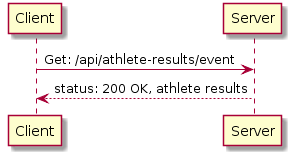
\includegraphics[scale=0.7]{images/get-athletes-api-call.png}
    \caption{GET kall for henting av utøvere}\label{fig:get-at-api}
\end{figure}

\begin{figure}[ht]
\centering 
    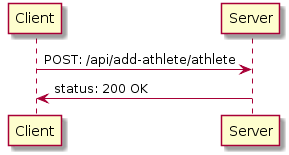
\includegraphics[scale=0.7]{images/post-athletes-api-call.png}
    \caption{POST kall for opplastning av utøvere}\label{fig:post-at-api}
\end{figure}
\end{document}
